\section{Topologie}
Nachdem in Kapitel \ref{sec:KonzeptionMeshNetz} ein Konzept für die Topologie entwickelt wurde folgt in diesem Unterkapitel die Beschreibung der Umsetzung des Mesh-Netzes, sowie der Allgemeine Aufbau der gesamten Topologie. 
\subsection{Allgemeine Beschreibung}
Die gesamte Projekt des Sensorknoten lässt sich fünf Ebenen unterteilen (siehe Grafik \ref{img:RealisierungTopologie}). Im den folgenden Abschnitten werden diese vier Schichten genauer erläutert.
\begin{figure}
	\centering
	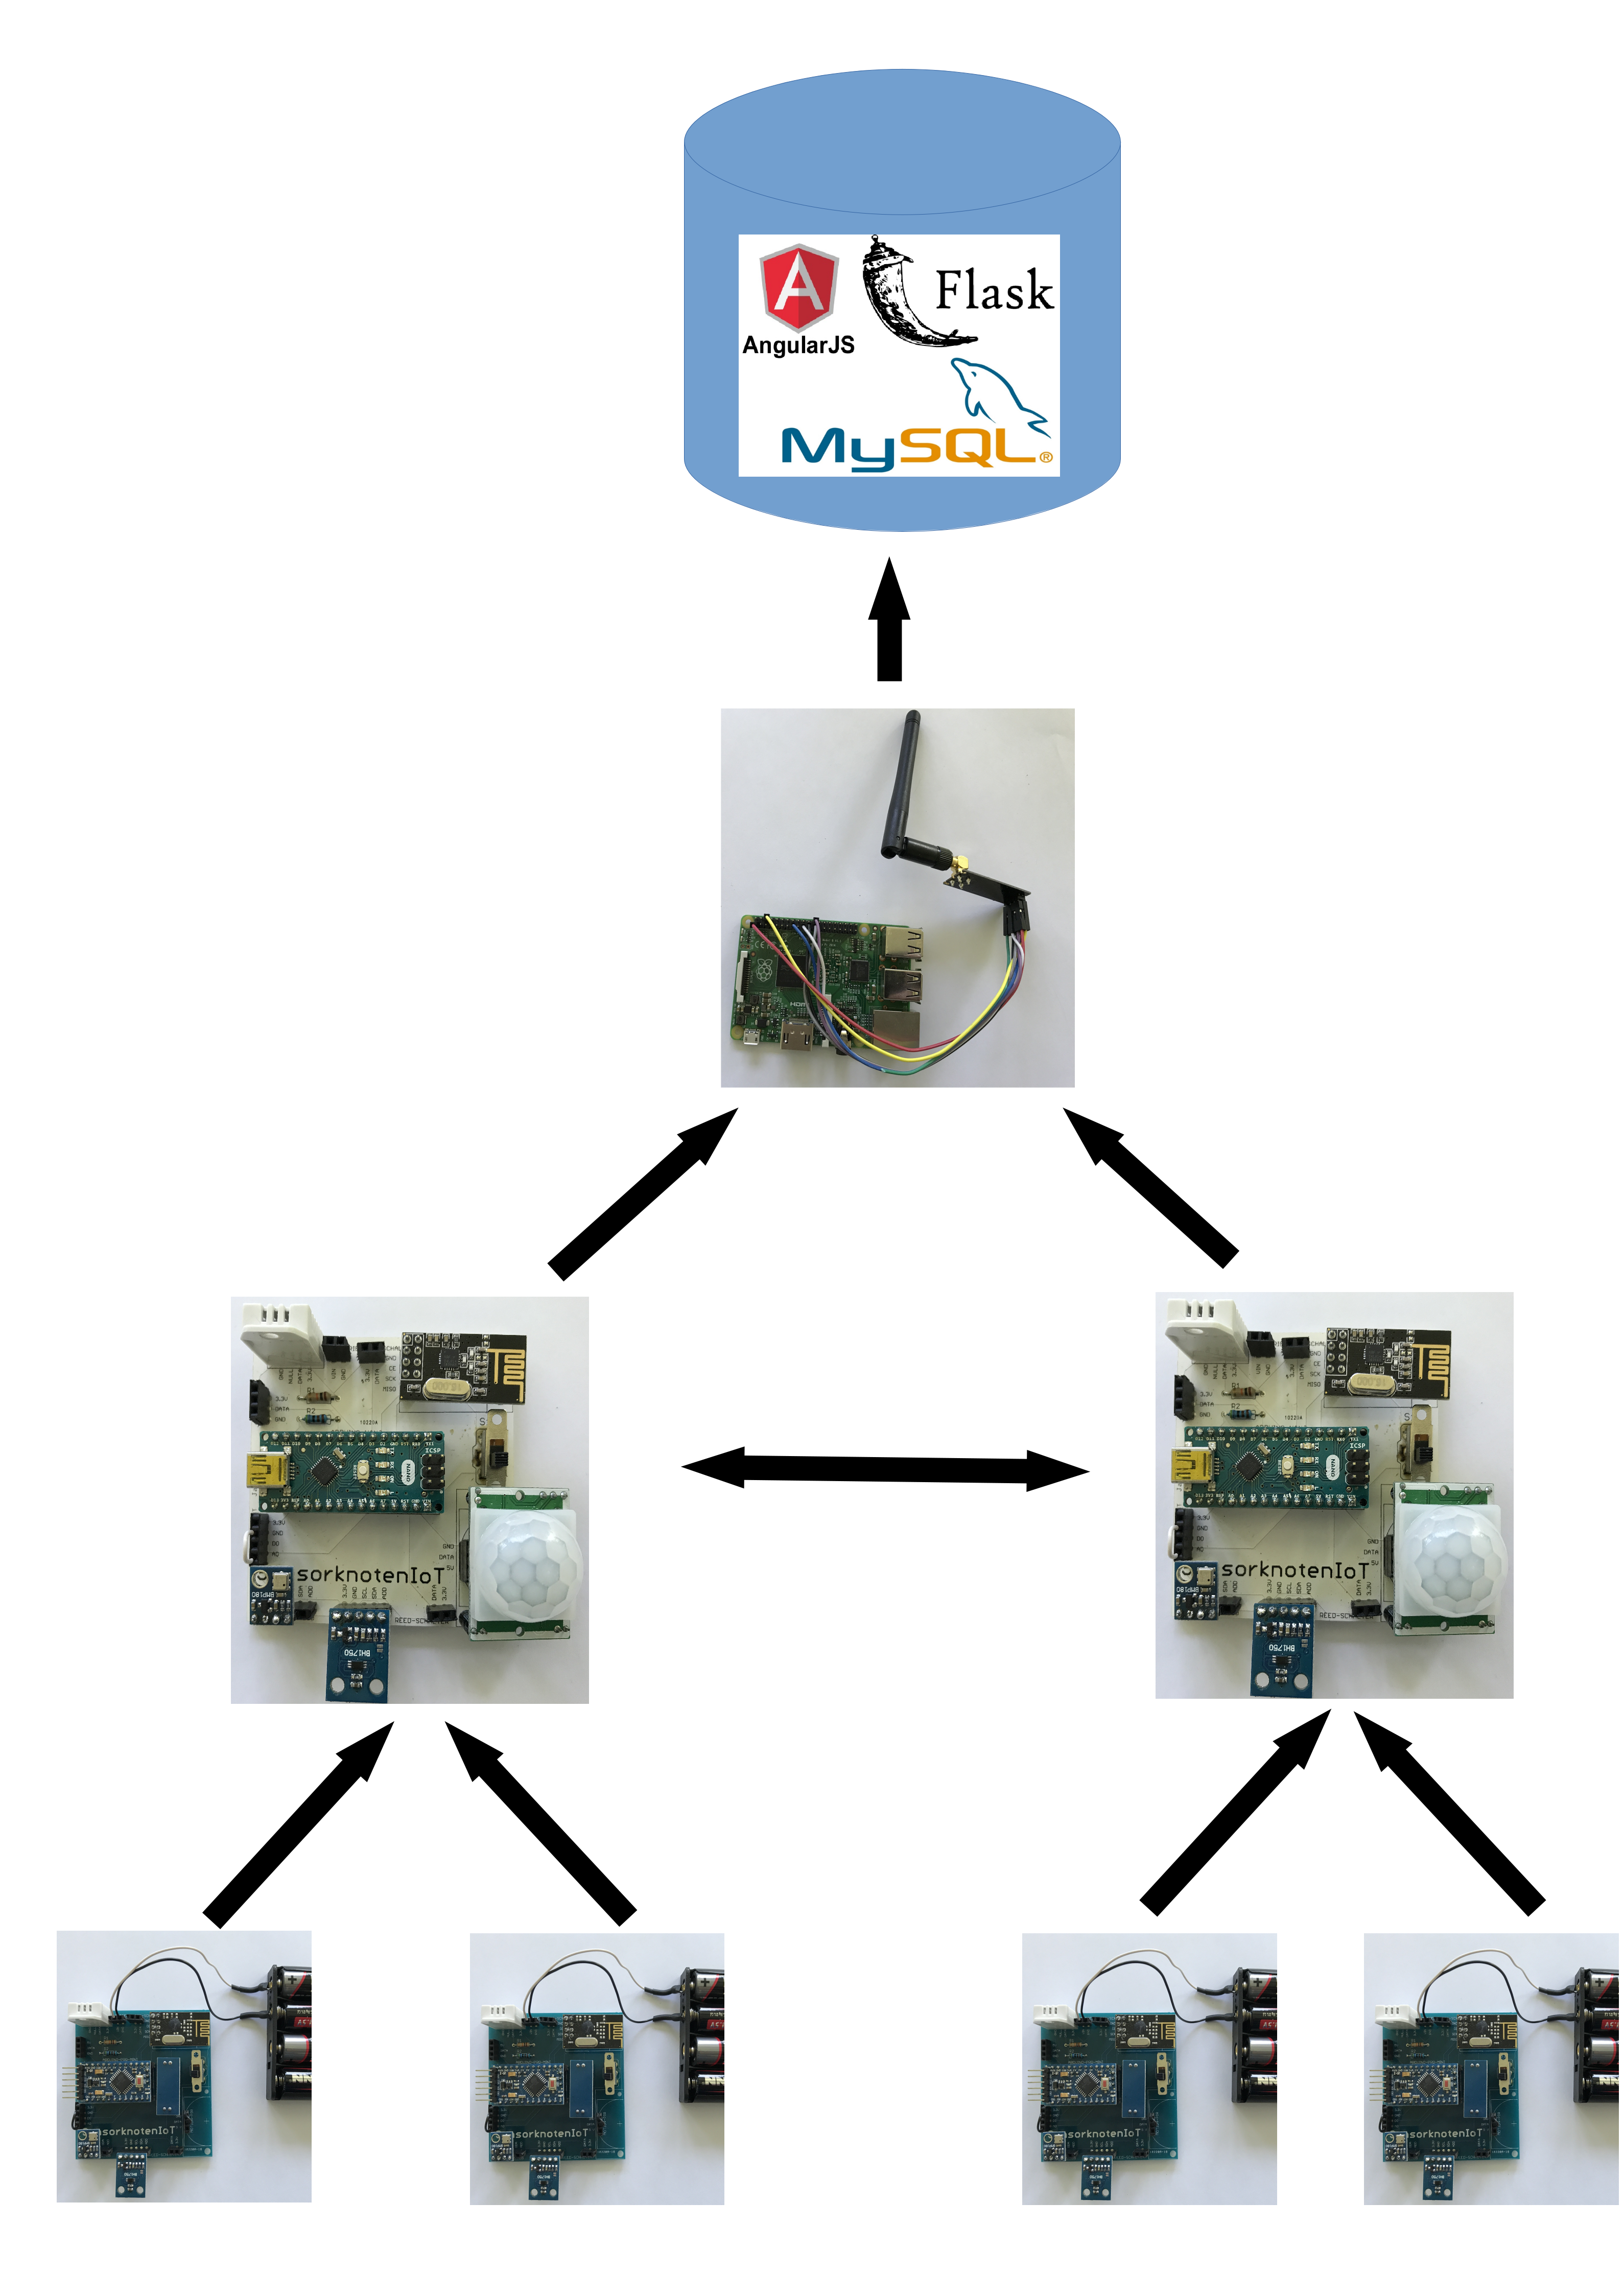
\includegraphics[width=0.7\textwidth]{bilder/topologie.png}
	\caption{Topologie Sensorknoten}
	\label{sec:KonzeptionMeshNetz}
\end{figure}
\paragraph{Energiesparender Sensorknoten} Der energiesparende Sensorknoten wurde mit einem Arduino Pro Mini realisiert. Dieser ist extrem Energiesparend und übernimmt keinerlei Weiterleitungsfunktion im Mesh-Netz. Dieser Sensorknoten sendet seine Daten entweder direkt dem Raspberry Pi oder einem normalen Sensorknoten, der die Nachricht dann zum Raspberry Pi weiterleitet. Auf den genauen Aufbau des energiesparenden Sensorknoten wird in Kapitel \ref{sec:ArduinoProMini} eingegangen.
\paragraph{Normaler Sensorknoten} Der normale Sensorknoten wird mit Hilfe eines Arduino Nano’s realisiert. Der Arduino Nano verfügt über eine permanente Stromversorgung, diese wird über den USB Port realisiert. Dieser Sensorknoten ist das Herz des Mesh-Netzes er übernimmt die Weiterleitung von Nachrichten im Netzwerk, zusätzlich bestimmt er jede Minute seine eigenen Messwerte. Diese werden dann ebenfalls entweder an einen weiteren normalen Sensorknoten weitergeleitet oder wenn der Raspberry Pi in der Nähe ist direkt an ihn. 
\paragraph{Gateway} Das Gateway zur Datenbank bzw. Internet wird mit einem Raspberry Pi realisiert. Dieser verfügt über das gleiche Funkmodul wie die beiden Sensorknoten mit dem Unterschied, dass das verwendete Funkmodul mit einer externen Antenne ausgestattet ist. Der Raspberry Pi verfügt zusätzlich über eine Verbindung zum Internet, diese kann wahlweise mit dem WLAN Modul erfolgen oder über Ethernet. In der DHBW wurde aufgrund von Probleme mit dem verwendeten Authenfizierungsprotokoll  Ethernet verwendet. Das genaue Vorgehen des Raspberry Pi’s nach dem erhalten der Nachricht wird in Kapitel \ref{sec:RaspberryPi} genauer betrachtet.
\paragraph{Datenhaltungsschicht} Der Raspberry Pi speichert die erhaltenen Daten in einer Datenbank. Diese Datenbank wird auf einem externen Server gehostet. Als relationales Datenbankverwaltungssystem wird MySQL eingesetzt. Der genaue Aufbau der Datenbank wird in Kapitel \ref{sec:Datenbankschema} betrachtet.
\paragraph{Datenvisualisierungsschicht} Nachdem die Daten erfolgreich in der Datenbank gespeichert wurden, können Sie mit Hilfe eines REST-Services aus dieser wieder extrahiert werden und auf eine Webseite dargestellt werden. Der REST-Service wurde mit dem Python Microframework Flask (siehe Kapitel \ref{}entwickelt. Der REST Service läuft auf einem NGINX (https://nginx.org/en/). Der REST Service kann von vielen verschiedenen Plattformen genutzt werden, so ist es möglich neben einer Webseite noch eine native App für Smartphones zu entwickeln. Die Webseite wird auf einem TomEE (http://tomee.apache.org/) gehostet. Die Frontend wurde mit AngularJS, HTML5, CSS3 und Bootstrap entwickelt. Die genaue Beschreibung der Visualisierung erfolgt in Kapitel \ref{sec:Datenvisualisierung}.
\subsection{Umsetzung des Mesh-Algorithmus}

-zuordnung aktiv/passiv
-schema mit bildern
-raspi anbindung an web
-code mesh netz
-Anpassung an lib für broadcast
